% Motivation — ReCAHS paper

\section{Motivation: Regime-Dependent Head Structure}
\label{sec:motivation}

\begin{figure*}[!tp]
  \centering
  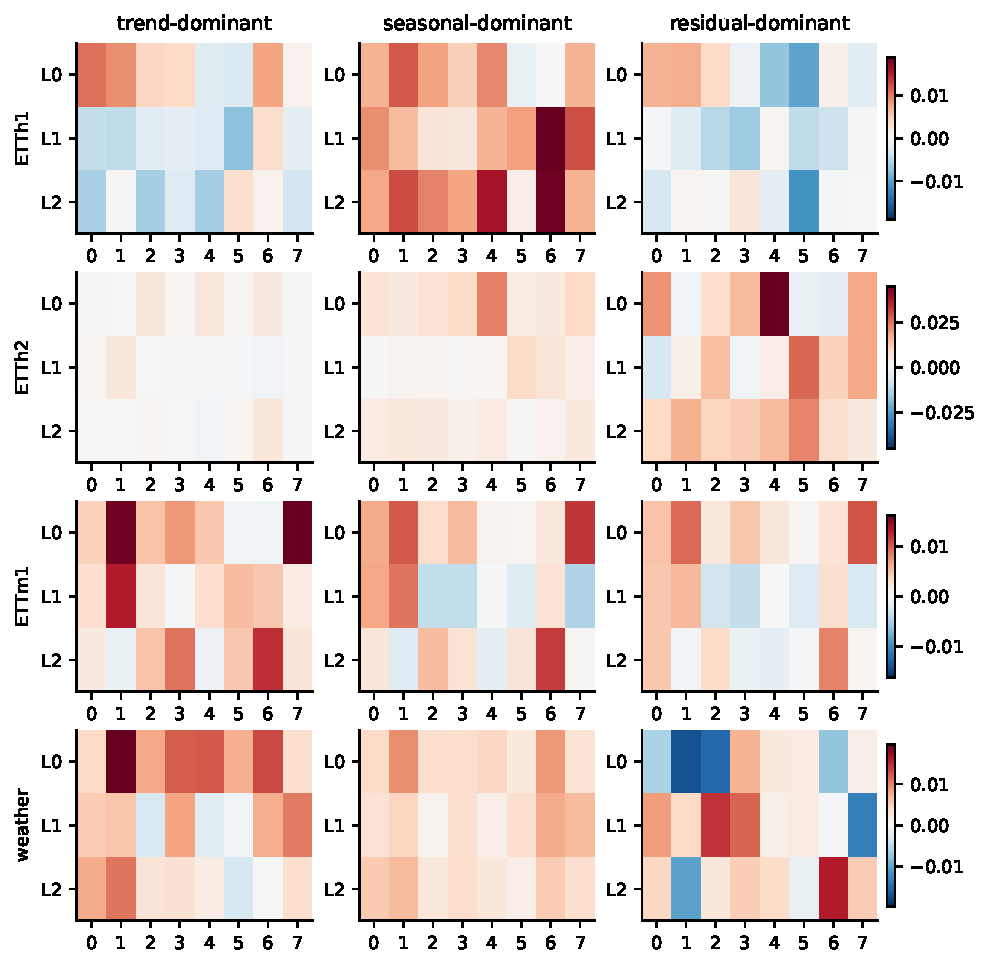
\includegraphics[width=\textwidth]{figures/fig_importance_heatmap.pdf}
  \caption{Leave-one-out head importance ($\Delta$ validation MSE when the
  head is removed; red $=$ removal hurts, blue $=$ removal helps),
  averaged over 5 seeds, per STL regime (columns) and dataset (rows) at
  horizon 96. Column-to-column differences within a row are the regime
  effect; on average $10.9$ of $24$ heads flip sign across regimes.}
  \label{fig:heatmap}
\end{figure*}

\begin{figure}[!htbp]
  \centering
  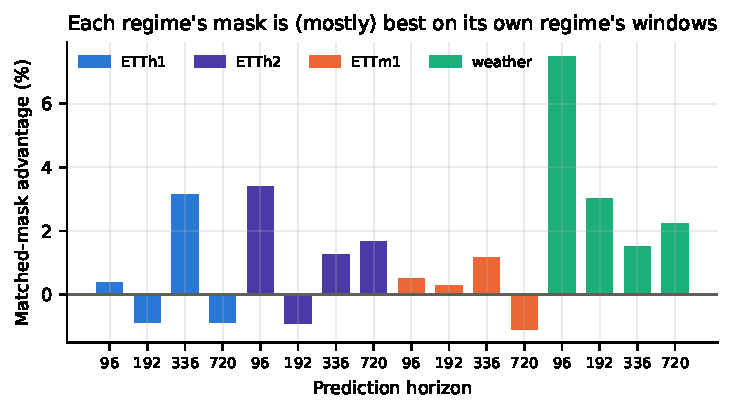
\includegraphics[width=\linewidth]{figures/fig_matched_advantage.pdf}
  \caption{Matched-mask advantage: relative error reduction of each
  regime's specialist mask on its own regime's test windows compared with
  the other regimes' masks ($25\%$ sparsity, mean over 5 seeds). Positive
  in $12/16$ cells; on Weather in all seed-cells.}
  \label{fig:matched}
\end{figure}

Classical time-series analysis decomposes a series into trend, seasonal
and remainder components \citep{cleveland1990stl}, and regime-switching
models formalize the observation that the data-generating process itself
alternates between states \citep{hamilton1989regime}. If attention heads
specialize --- as they do in language models
\citep{voita2019analyzing} --- it is natural to ask whether their
usefulness in a forecasting Transformer depends on which temporal regime
the input window is in.

Three preliminary observations motivate the study
(Fig.~\ref{fig:heatmap}). First, within a trained PatchTST model, an
average of $10.9$ of $24$ heads \emph{flip the sign} of their
leave-one-out importance across STL-labeled regimes: removing such a head
hurts trend-dominant windows but helps residual-dominant ones, or vice
versa. Second, this structure is causally exploitable: a mask selected
for regime $r$ achieves lower error on regime-$r$ test windows than the
other regimes' masks in $12/16$ dataset$\times$horizon cells
(Fig.~\ref{fig:matched}), on weather in all $20/20$ seed-cells. Third,
the structure is model-specific: head importance \emph{rankings}
correlate strongly across regimes within one trained model
($\bar\tau_{\text{trend,seasonal}}{=}0.24$) but barely at all across
training seeds ($\bar\tau{\approx}0.05$) --- which head plays which role
is an accident of training, so any selection procedure must operate
per model rather than transfer masks between models.

These observations make regime-conditional head selection plausible, but
they do not establish that it \emph{works}: a regime-routed method could
gain from better selection rather than from routing, and per-window
regime structure could be too noisy to exploit at inference time. The
study is therefore organized around three questions:
\begin{itemize}
  \item \textbf{Q1 (criterion).} How much of head-pruning quality is
  determined by the selection criterion alone --- independent scoring
  vs.\ joint greedy elimination --- across sparsity levels?
  \item \textbf{Q2 (conditioning).} Holding the criterion fixed, does
  conditioning the selection and its deployment on the detected regime
  add test-time accuracy?
  \item \textbf{Q3 (headroom).} How large is the gap between deployable
  regime-conditional methods and a per-window oracle over the same
  masks, and can any inference-time-legal mechanism close it?
\end{itemize}
